\documentclass[12pt]{amsart}
\usepackage{geometry} % see geometry.pdf on how to lay out the page. There's lots.
\usepackage{graphicx}	% Including figure files
\usepackage{amsmath}	% Advanced maths commands
\usepackage{amssymb}	% Extra maths symbols
\usepackage{hyperref}
\usepackage{float}
\geometry{a4paper} % or letter or a5paper or ... etc

\title{CSE 546: Machine Learning Homework 2}
\author{David P. Fleming}
\date{October 28$^{th}$, 2016}

%%% BEGIN DOCUMENT
\begin{document}

\maketitle
\tableofcontents

\section*{Introduction}

Please note that a copy of all the code I wrote to answer the questions in this assignment are included in my submission but also located online at \url{https://github.com/dflemin3/CSE_546/tree/master/HW2}.  Some scripts require data, such as MNIST data, to run to completion and were not included on my github or in my submission due to file size constraints.  If requested, I will happily send a compressed directory containing my homework and detailed instructions on how to reproduce my work.  My primary email is dflemin3 (at) uw (dot) edu.  Also for reproducibility, I set the random number generator seed near the top of each script such that rerunning my script will yield the same answers as presented here.

%%% QUESTION 1 %%%

\section*{Question 1: TODO}
TODO

%%% QUESTION 2 %%%
\section*{Question 2: Multi-Class Classification using Logistic Regression and Softmax}

The code used to answer this question and all subquestions are contained within the following python files: {\tt classifier$\_$utils.py, validation.py, gradient$\_$descent.py, mnist$\_$utils.py, hw2$\_$2.1.py}.

\subsection*{2.1: Binary Logistic Regression}

For this question, I filtered the MNIST data such that all Y digits equal to 2 were set to 1 and all other labels set to 0 to make this a binary classification problem.  I trained a logistic regression model on the MNIST training data using regularized batch gradient ascent to maximize the log-likelihood of the data as defined in class notes as
\begin{equation} \label{eqn:loglike}
LL = \sum_j [y^j (w_0 + \sum_{i=1}^d X_i^j \hat{w}_i) - \log(1+ \exp(w_0 + \sum_{i=1}^d X_i^j \hat{w}_i))].
\end{equation}
Maximizing Eqn.~\ref{eqn:loglike} over the training set then yields the predicted parameters $\hat{w}, w_0$.  For all fits, I chose a batch size of 6,000, or 10$\%$ of the training data for computational speed gains.  I called my solution converged once the log-likelihood changed by less than $0.5 \%$.  I varied my convergence threshold and tested smaller values and found comparable performance.

For my regularized batch gradient ascent implementation, I used the $l_2$ norm penalty as was derived in class.  When fitting this algorithm, I need to optimize of the following hyperparameters: the learning rate $\eta$ and the regularization constant $\lambda$.  The hyperparameters of my model were simultaneously fit for along a regularization grid.  Since my training set was sufficiently large with $N = 60,000$ samples, I randomly partitioned it into a validation set with $N_{val} = 6,000$ and a training set with $N_{train} = 54,000$.  I iterated over a two-dimensional grid of $\eta \in [0.001,100]$ in 6 logarithmic bins and $\lambda \in [10^{-3},10^{3}]$ in 6 logarithmic bins.  For each $(\eta,\lambda)$ pair, I ran batch gradient ascent on the training set then tested it on the validation data.  I used the validation predictions to compute the log-likelihood and stored it for each grid point.  I found the optimal $\eta = 0.001$ and $\lambda = 10^3$ from the maximum value of the log-likelihood grid.  

\subsubsection*{2.1.1}

As discussed above in my description of how I optimized my hyperparameters, I found $\eta = 0.001$ allows for the best fit.  In practice in my algorithm, I set $\eta = k\eta/N$ where $N$ is the number of samples fit over in a given batch and $k = 1/t$ is a scaling constant where $t$ is the iteration number.  I found that the inclusion of $k$ which tends to suppress later step sizes prevented the solution from bouncing around optima and instead allowed for more runs to converge.  In practice, $k$ could also slow down convergence by reducing the step size even if the solution was tending towards the correct global optimum but I found that this was not too big of a problem.

\subsubsection*{2.1.2}

With my optimal hyperparameters, I refit the batch gradient ascent on the entire $N = 60,000$ sample training set to get the final fit parameters $w_0$ and $\hat{w}$.  At each iteration of this fit, I computed the log-loss = -log-likelihood for both the training and testing set and plotted them in Fig.~\ref{fig:mnist_ll} below.

TODO.  Note: I did 01 loss for reg path and I wanted to minimize that...rerun 

\begin{figure}[H]
	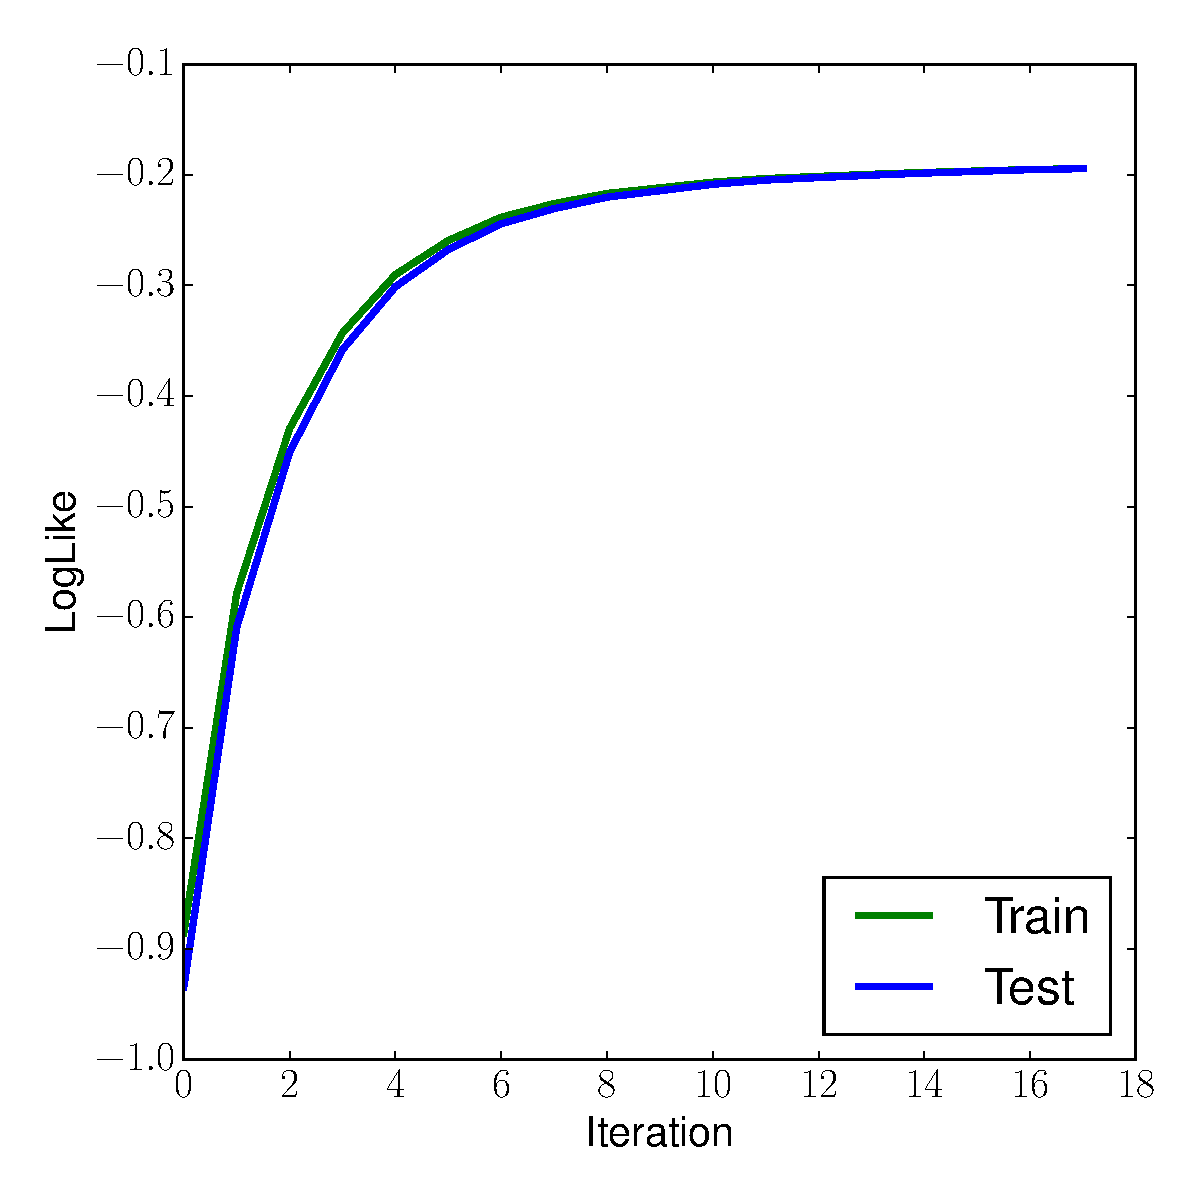
\includegraphics[width=\columnwidth]{mnist_train_test_ll.pdf}
    \caption{Log loss as a function of iteration for both the MNIST training and testing datasets.  The log loss on the testing set was evaluated using the model parameters computed by fitting on the training set for each iteration.  Note how the loss decreases for both sets with each iteration as the fit improves.  In general, the testing loss is slightly larger than the training loss as expected.}
    \label{fig:mnist_ll}
\end{figure}

\subsubsection*{2.1.3}
TODO

Note: On this question, I collaborated with Matt Wilde, Serena Liu, and Janet Matsen.

\end{document}